\section{Background}
\subsection{Other Technologies}

There are other technologies that can produce contactless forces between a spacecraft and a target. Coulomb force has been shown to produce useful interactions between two charged spacecraft as long as the distance between them is less than the Debye length. \cite{coulombtether} A number of different systems produce contactless forces with magnetic interactions among controlled dipoles on both the spacecraft and the target.\cite{dipoleplanning} \cite{Kong2004}
All such approaches place requirements for specific hardware on both the chaser and the target (that is, the target must have launched with certain features already in place.) Implementing these systems is not standard practice, and in fact no spacecraft currently in orbit are known to include components designed for contactless grappling through such techniques.

Laser tweezers can produce contactless force on an uncooperative target. \cite{lasertweezers}However, the tweezers are best at manipulating micron- scale particles, a size restriction that no spacecraft beyond Technology Readiness Level (TRL) $1$ can meet. \cite{lasermirrors} Thruster plumes can also produce forces between a chaser and a target. However, typically the combustion products from thrusters carry significant risk of contaminating optical instruments and solar panels, among other disadvantages. We conclude that current technology is limited to direct mechanical contact as the only general solution for manipulating a target that has not been designed to be cooperative.  This limitation motivates the present study.

\subsection{Induced Current Force}

Eddy-current force starts with a time-varying magnetic field. The field induces an electrical eddy current in any conductive material nearby. In turn, that induced current interacts with the original magnetic field, producing force between the conductive material and the source of the magnetic field.

The currents in the conductor depend on the geometry of the target, its conductivity, $\sigma$, the direction and magnitude of both \textbf{B} and $\frac{d\textbf{B}}{dt}$, and the velocity and position of the induction coupler relative to the target. Compounding the subtlety is the unavoidable coupling between the magnetic field and the kinematics of the magnets in the induction coupler. These interdependencies make the force sensitive to the state of the system. Induction couplers exhibit many nonlinearities, which demand a rigorous and informed approach to implementing the technology.

Eddy-current force is a consequence of Maxwell's equations:

\begin{equation}\label{eq:FaradayInduction}
\nabla \times \textbf{E} = -\frac{d\textbf{B}}{dt}
\end{equation}
\begin{equation}\label{eq:AmperesLaw}
\nabla \times \textbf{B} = \mu_0 \textbf{J}
\end{equation}
\begin{equation}\label{eq:GaussLaw}
\nabla \cdot \textbf{B} = 0
\end{equation}
Any material with finite conductivity experiences a voltage gradient in response to a time-varying magnetic field. 
\begin{equation}\label{eq:currentflow}
\textbf{J}=\sigma \textbf{E}
\end{equation}

The voltage difference induces a current in the material that in turn generates its own magnetic field. The resulting field has a vector potential that obeys 
\begin{equation}\label{eq:vectorPotential}
\textbf{B} = \nabla \times \textbf{A}
\end{equation}
\begin{equation} \label{eq:Efield}
\textbf{E} =  -\frac{d\textbf{A}}{dt} - \nabla V
\end{equation}

If the conductive plate is linear and simply connected, the governing equations can be combined into a partial differential equation describing the propagation of $\textbf{A}$ through the plate \cite{Smyth1989}

\begin{equation}\label{eq:governingPDE}
\nabla^2 \textbf{A} = \mu_0\sigma \frac{d\textbf{A}}{dt}
\end{equation}
Once \textbf{A} is known on the surface of the plate, Maxwell's stress tensor solves for the force between the plate and the magnetic source. Because there is no electric field exterior to the plate, Maxwell's stress tensor ($\overset{\leftrightarrow  }{ \mathbf{\sigma} }$) reduces to
\begin{equation} \label{eq:stressTensor}
\overset{\leftrightarrow  }{ \mathbf{\sigma} } = \frac{1}{\mu_0} \left[ \mathbf{B}\otimes\mathbf{B} - \frac{B^2 }{2} (\mathbf{\hat x}\otimes\mathbf{\hat x} + \mathbf{\hat y}\otimes\mathbf{\hat y} + \mathbf{\hat z}\otimes\mathbf{\hat z}) \right]
\end{equation}

%" src="//upload.wikimedia.org/math/8/d/e/8dea2b36115634afa876918c145f67bf.png">

% TODO Update this figure - make the vectors correct, perhaps make isometric
\begin{figure}
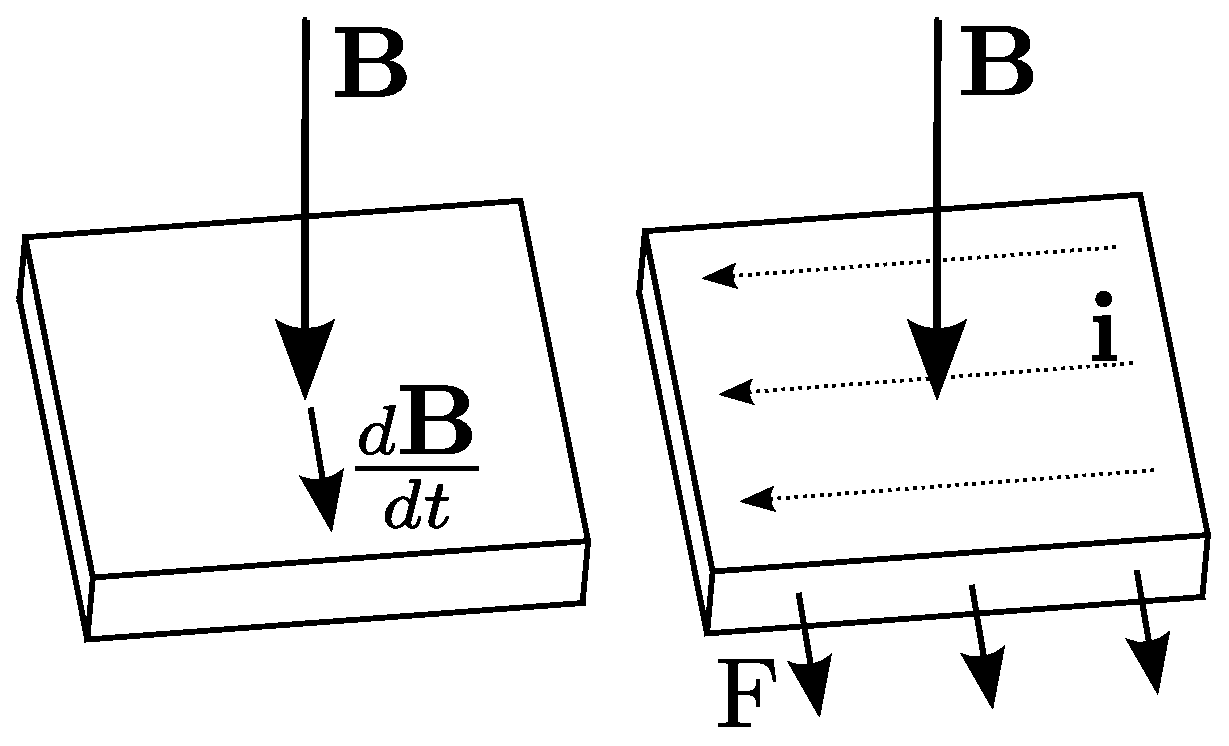
\includegraphics[width = 6cm, height = 6cm ]{figures/iso_force_creation.eps}
\label{fig:force_generation}
\caption{Creating graphical intuition for the problem - a magnetic field directed into the conductor changes in the upward direction. This change induces a current to the left that interact with the original B field to create a downward force.}
\end{figure}

There are many ways to find the magnetic potential in the plate and its resultant actuation force, but few of them are suitable for a model that includes feedback control and rigid-body dynamics. \cite{Paudel2013}
Finite element methods are the standard approach to solving this class of problems quasistatically. However, even those few commercially available FEM packages that can account for a moving source field are computationally expensive and require hand-tuning for each new geometries. These drawbacks make them unsuitable for the dynamical simulations necessary for online control. 

There are also several analytical models for eddy-current forces, but most are also unsuitable for dynamical systems. Most of these models do not take into account a moving source field, which is an essential part of a dynamic system. All analytical solutions to the partial differential equation describing eddy-current propagation are tied to specific geometries. This is not inherently a problem, but most of the assumptions about the orientation of the field are too restrictive to be useful in a dynamic system that can move in 6 DoF near the conductive surface. 

Paudel and Bird introduced an analytical model that both relaxes the geometry restrictions and accounts for a moving magnetic source. Their method finds transient force between a time-varying, moving magnetic source field and a large flat conductive plate. \cite{Paudel2012t}
This model can also be simplified to a computationally-lightweight steady-state solution that finds the force from a magnetic field with a single frequency component. \cite{Paudel2012ss}
The steady-state model is a good approximation when 
\begin{enumerate}
\item There are no interactions between the fields of multiple magnet arrays. 
\item The mechanical frequencies are much lower than the propagation speed of the magnetic field through the conductor.
\item The changing magnetic field has only one frequency component.
\end{enumerate}
This paper uses the steady-state Paudel and Bird method to model the force from the spinning magnet arrays in an induction coupler. 
 
%% TODO THIS PARAGRAPH NEEDS TO BE TRUTHIFIED
Systems of induction couplers can produce force in any direction relative to the target, for example both tangential and perpendicular to a surface on that target. Therefore, a chaser spacecraft generating a time-varying magnetic field can produce forces in all three translational degrees of freedom. Two induction couplers separated by a moment arm can also produce torques, for complete 6DoF actuation.
%% TODO - move this. Perhaps include figures for this. 
There are two ways for an induction coupler to generate its changing magnetic fields and resultant force: permanent magnets that move mechanically and electromagnets driven by time-varying currents. Each type of magnet is especially good at producing forces in different directions. For example, a single electromagnet with a sinusoidal driving current always repels the target. \cite{Reinhardt2012}.  A rotating permanent magnet is effective in producing a shear force, i.e. a force that lies in the plane of a surface.  Replicating the pure repulsive force of an electromagnet with a permanent magnet would require either a linear actuator or a complicated set of linkages. Therefore, a spacecraft that implements induction couplers likely incorporates a combination of permanent magnets and electromagnets..  This paper focuses primarily on a free-flyer inspection vehicle which uses those shear forces to move along its target. 